
\section{Results and Analysis}

The PGA hazard maps have been computed for a 10\% and 2\% exceedance probability in 50 years, corresponding to a return period of 475 and 2475 years, from gridded values of historical and instrumental seismic activity. These levels of exceedance are a standard practice in seismic designs \citep{BHRC2014}.

\begin{figure*}[t]
    \centering
    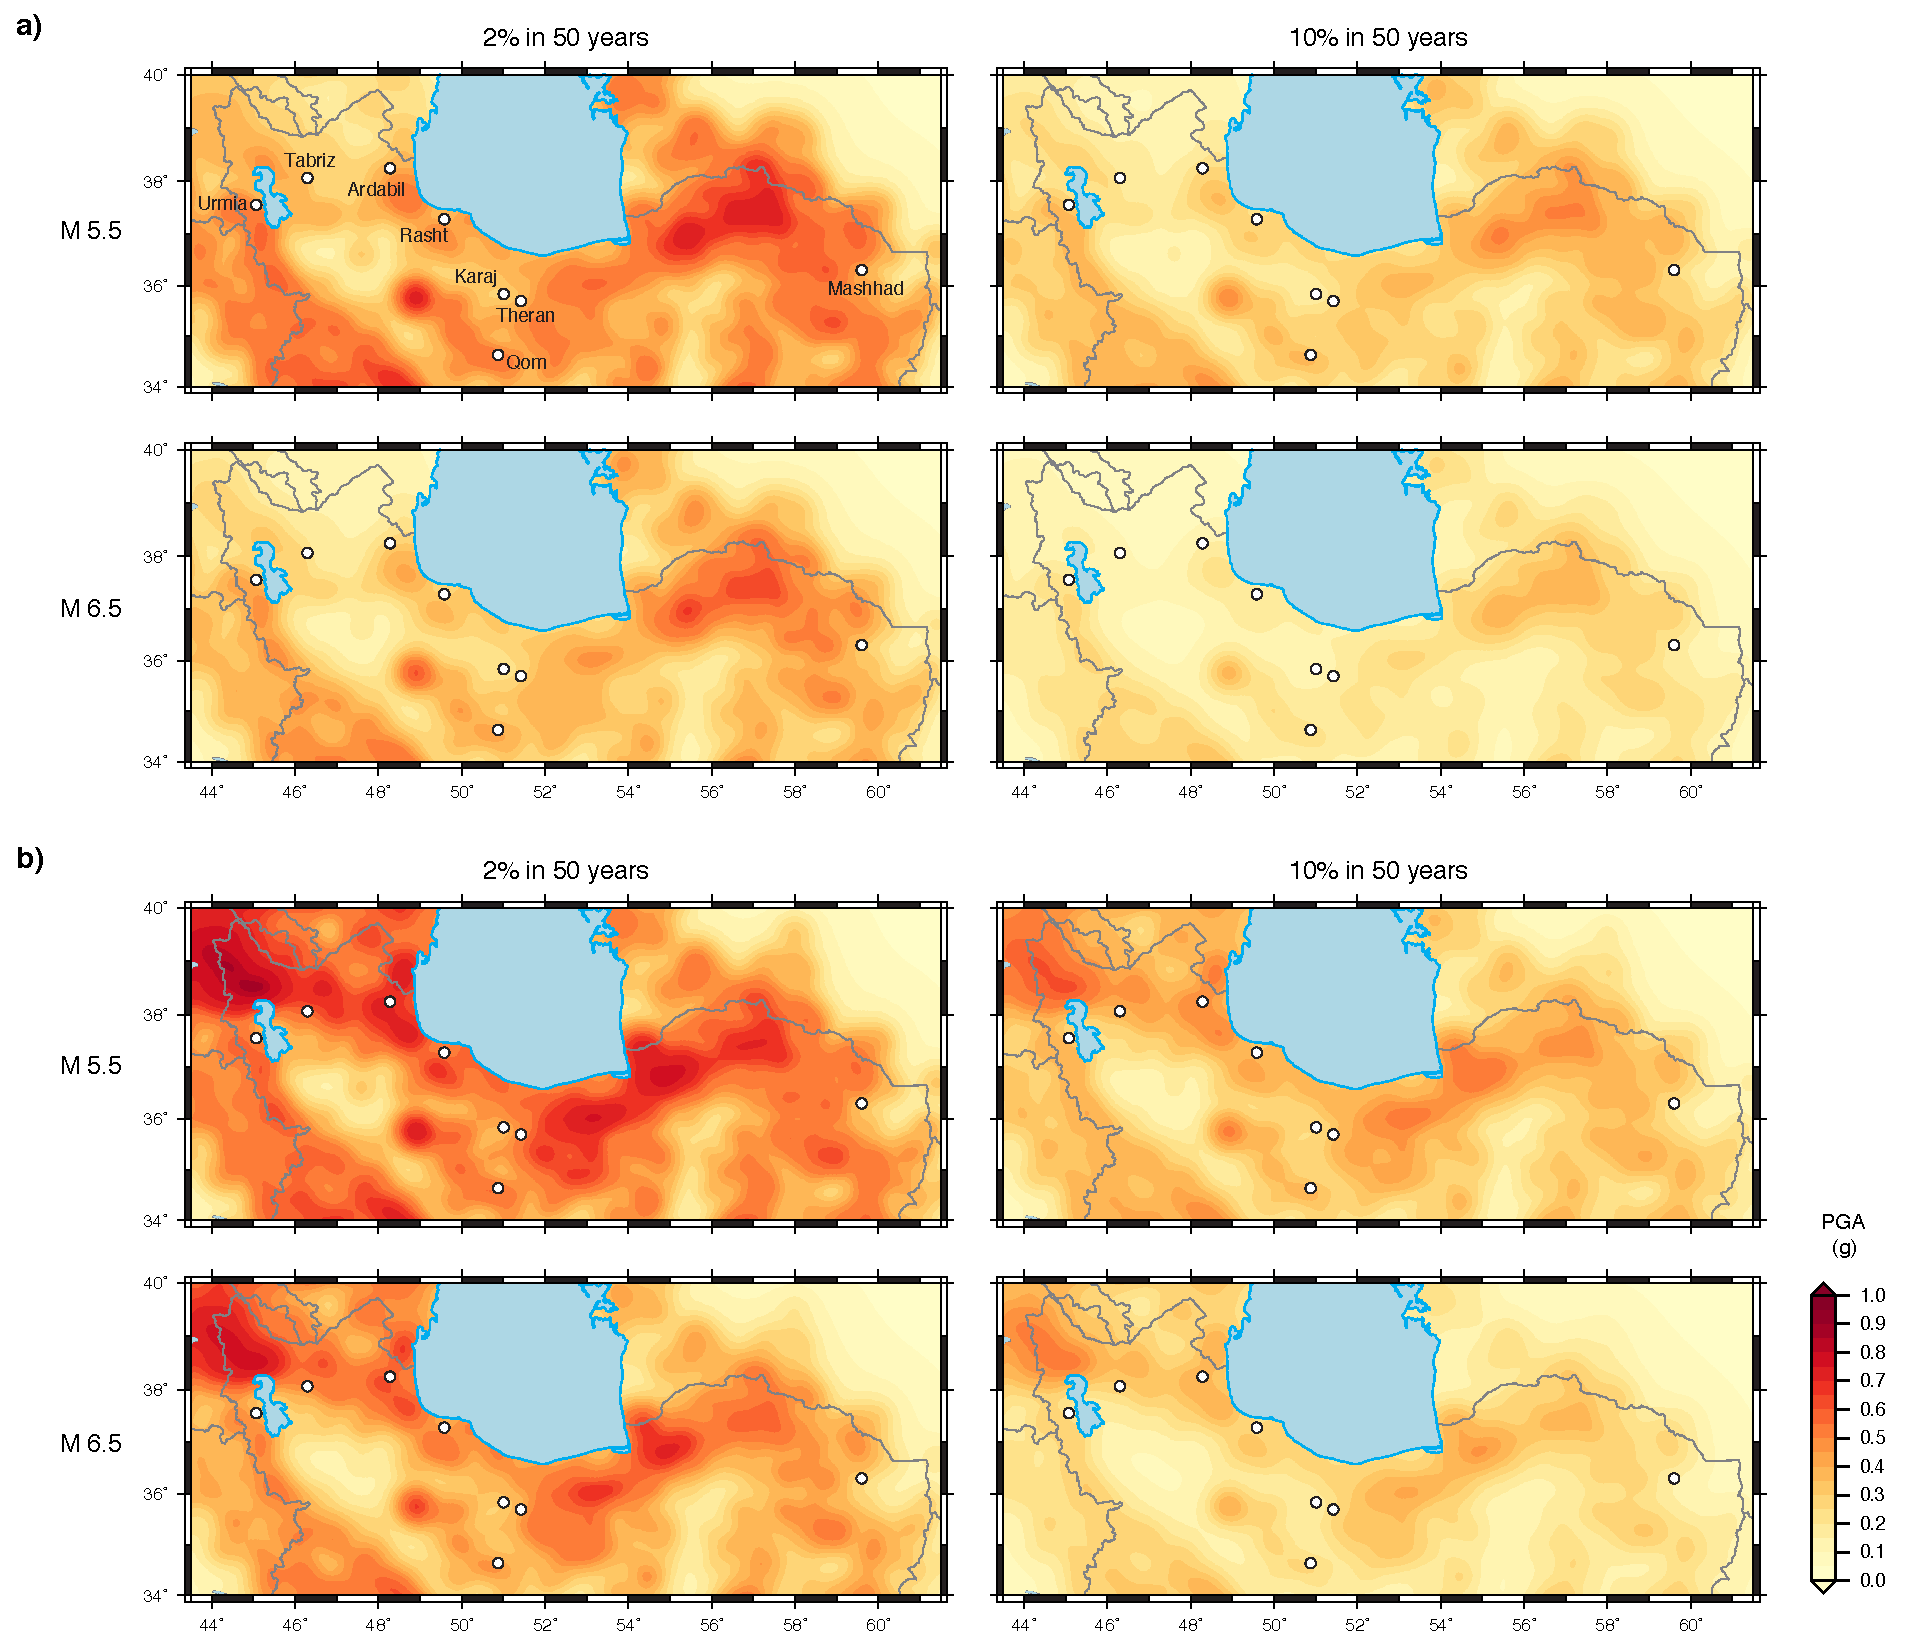
\includegraphics[width=\textwidth]{figures/pdf/figure-08.pdf} 
    \caption{PGA exceedance.}
    \label{fig:pga}
\end{figure*}

\begin{figure*}[t]
    \centering
    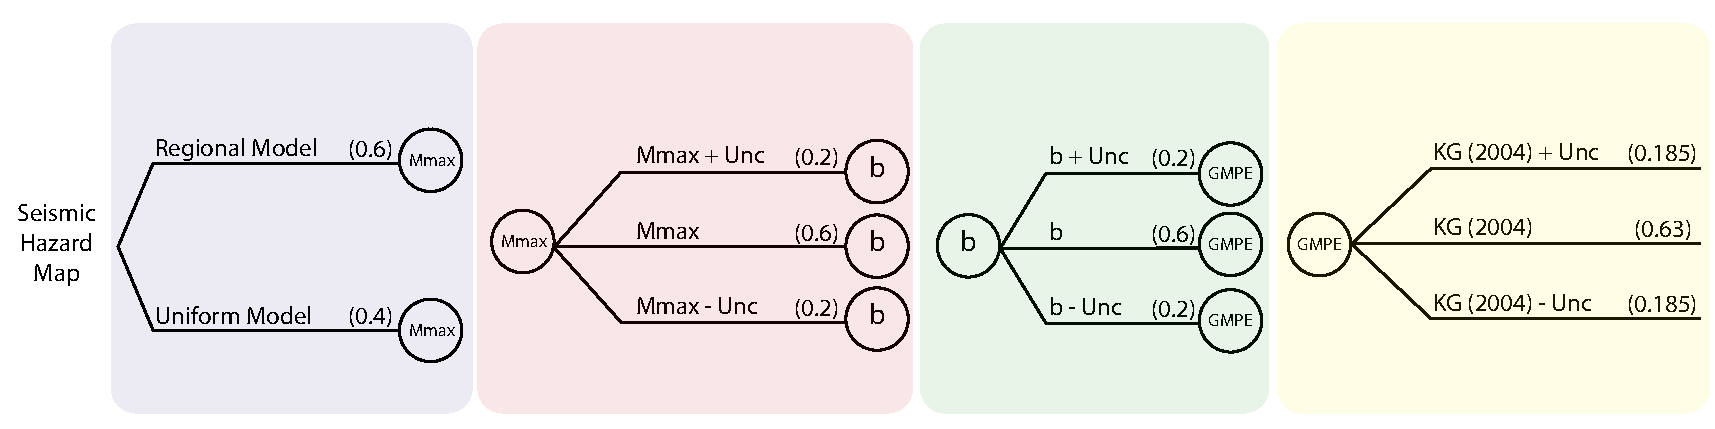
\includegraphics[width=\textwidth]{figures/pdf/figure-09.pdf} 
    \caption{Uniform minus zones.}
    \label{fig:pga}
\end{figure*}

\begin{figure*}[t]
    \centering
    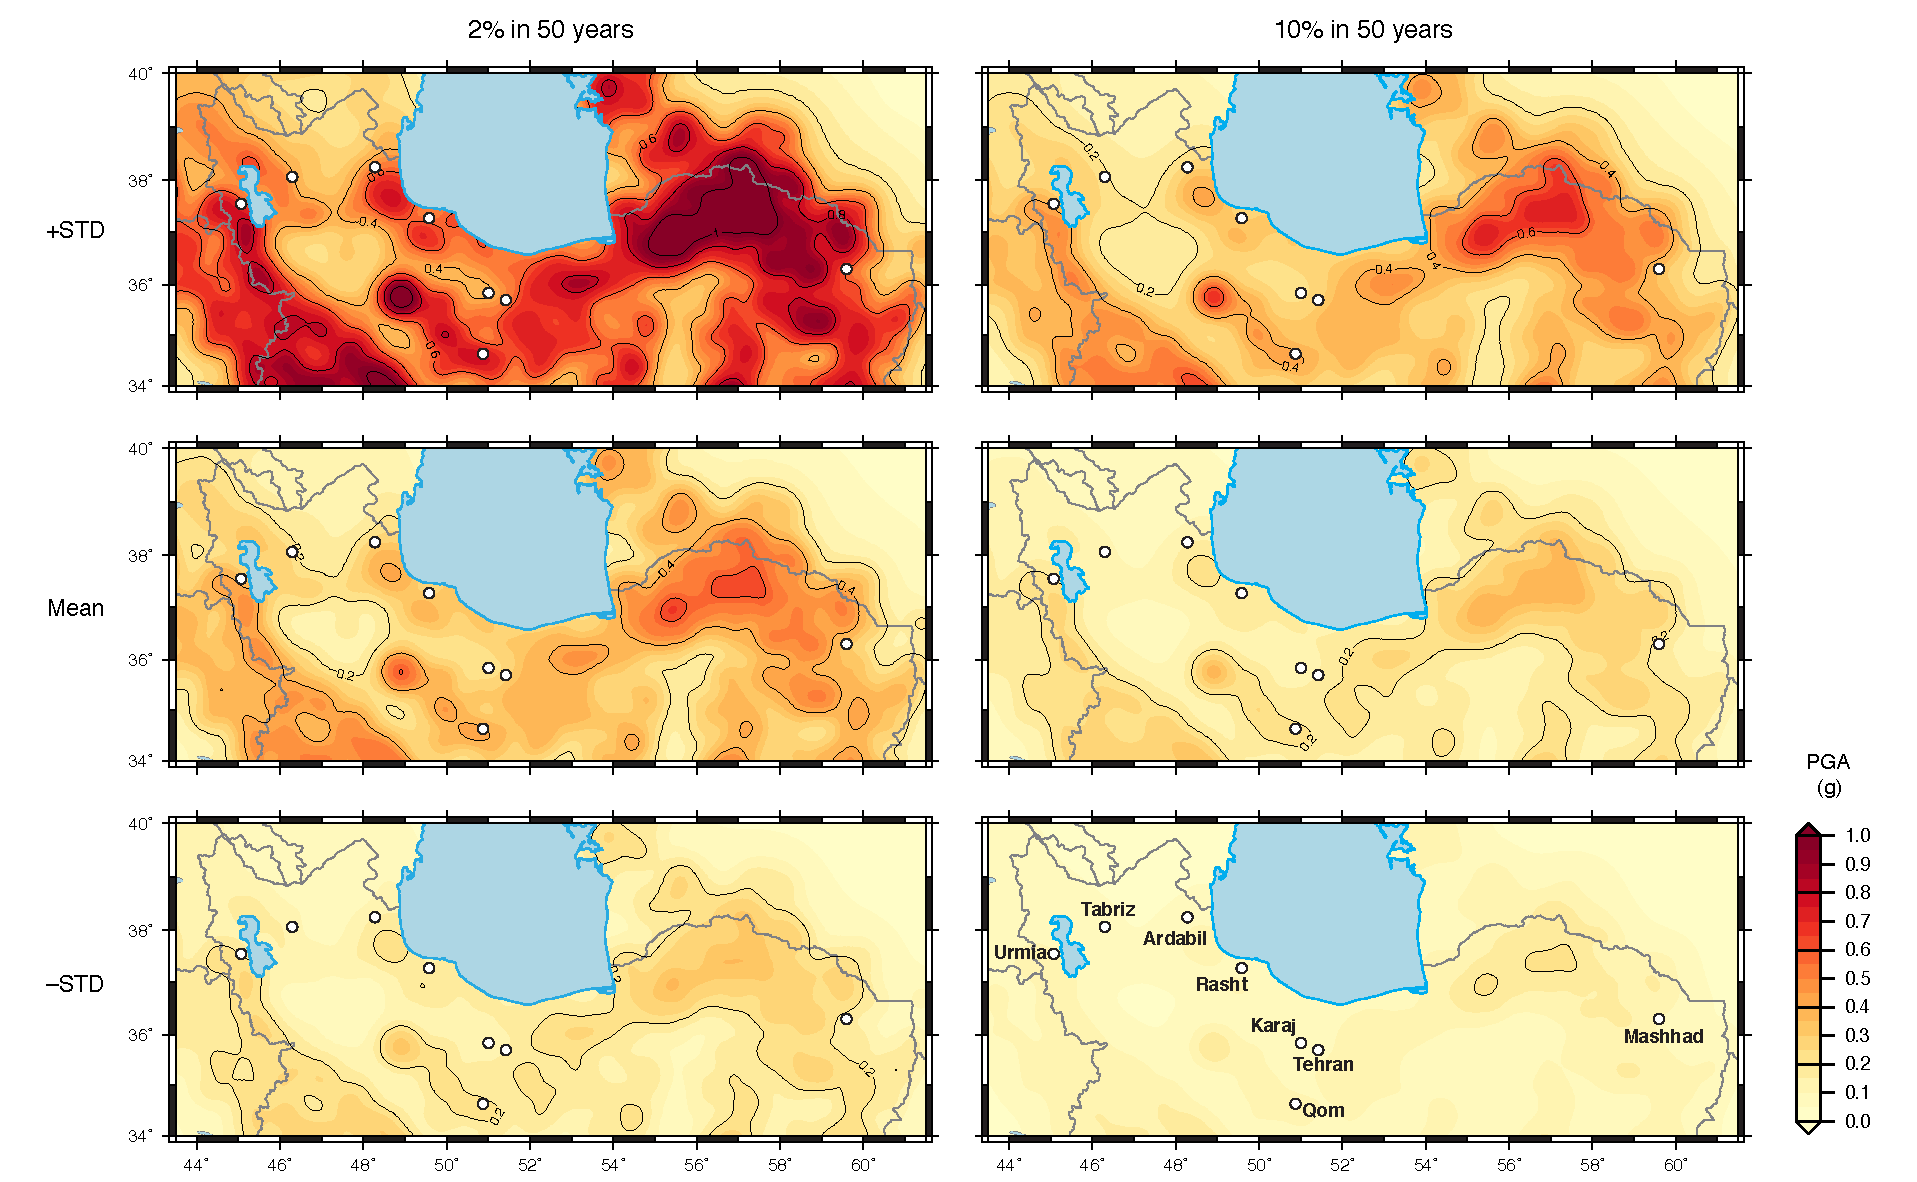
\includegraphics[width=\textwidth]{figures/pdf/figure-10.pdf} 
    \caption{plus minus std for M6.5.}
    \label{fig:pga}
\end{figure*}

Regarding the study domain and the 0.1 grid size, the total number of source as grid points is 13561. 

% \subsection{Hazard Curve}

We calculated the probability of exceedance of the ground motion from different ground motion levels, separately for each of 5 regions. We add the probability of all regions in order to have the effect of seismicity from all tectonic seismic regions. The results are presented as annual rate of exceedance. Fig.~\ref{fig:hazardcurve} represents the hazard curve of different model for some of important northern cities in Iran. 

\begin{figure*} [!ht]
\centering
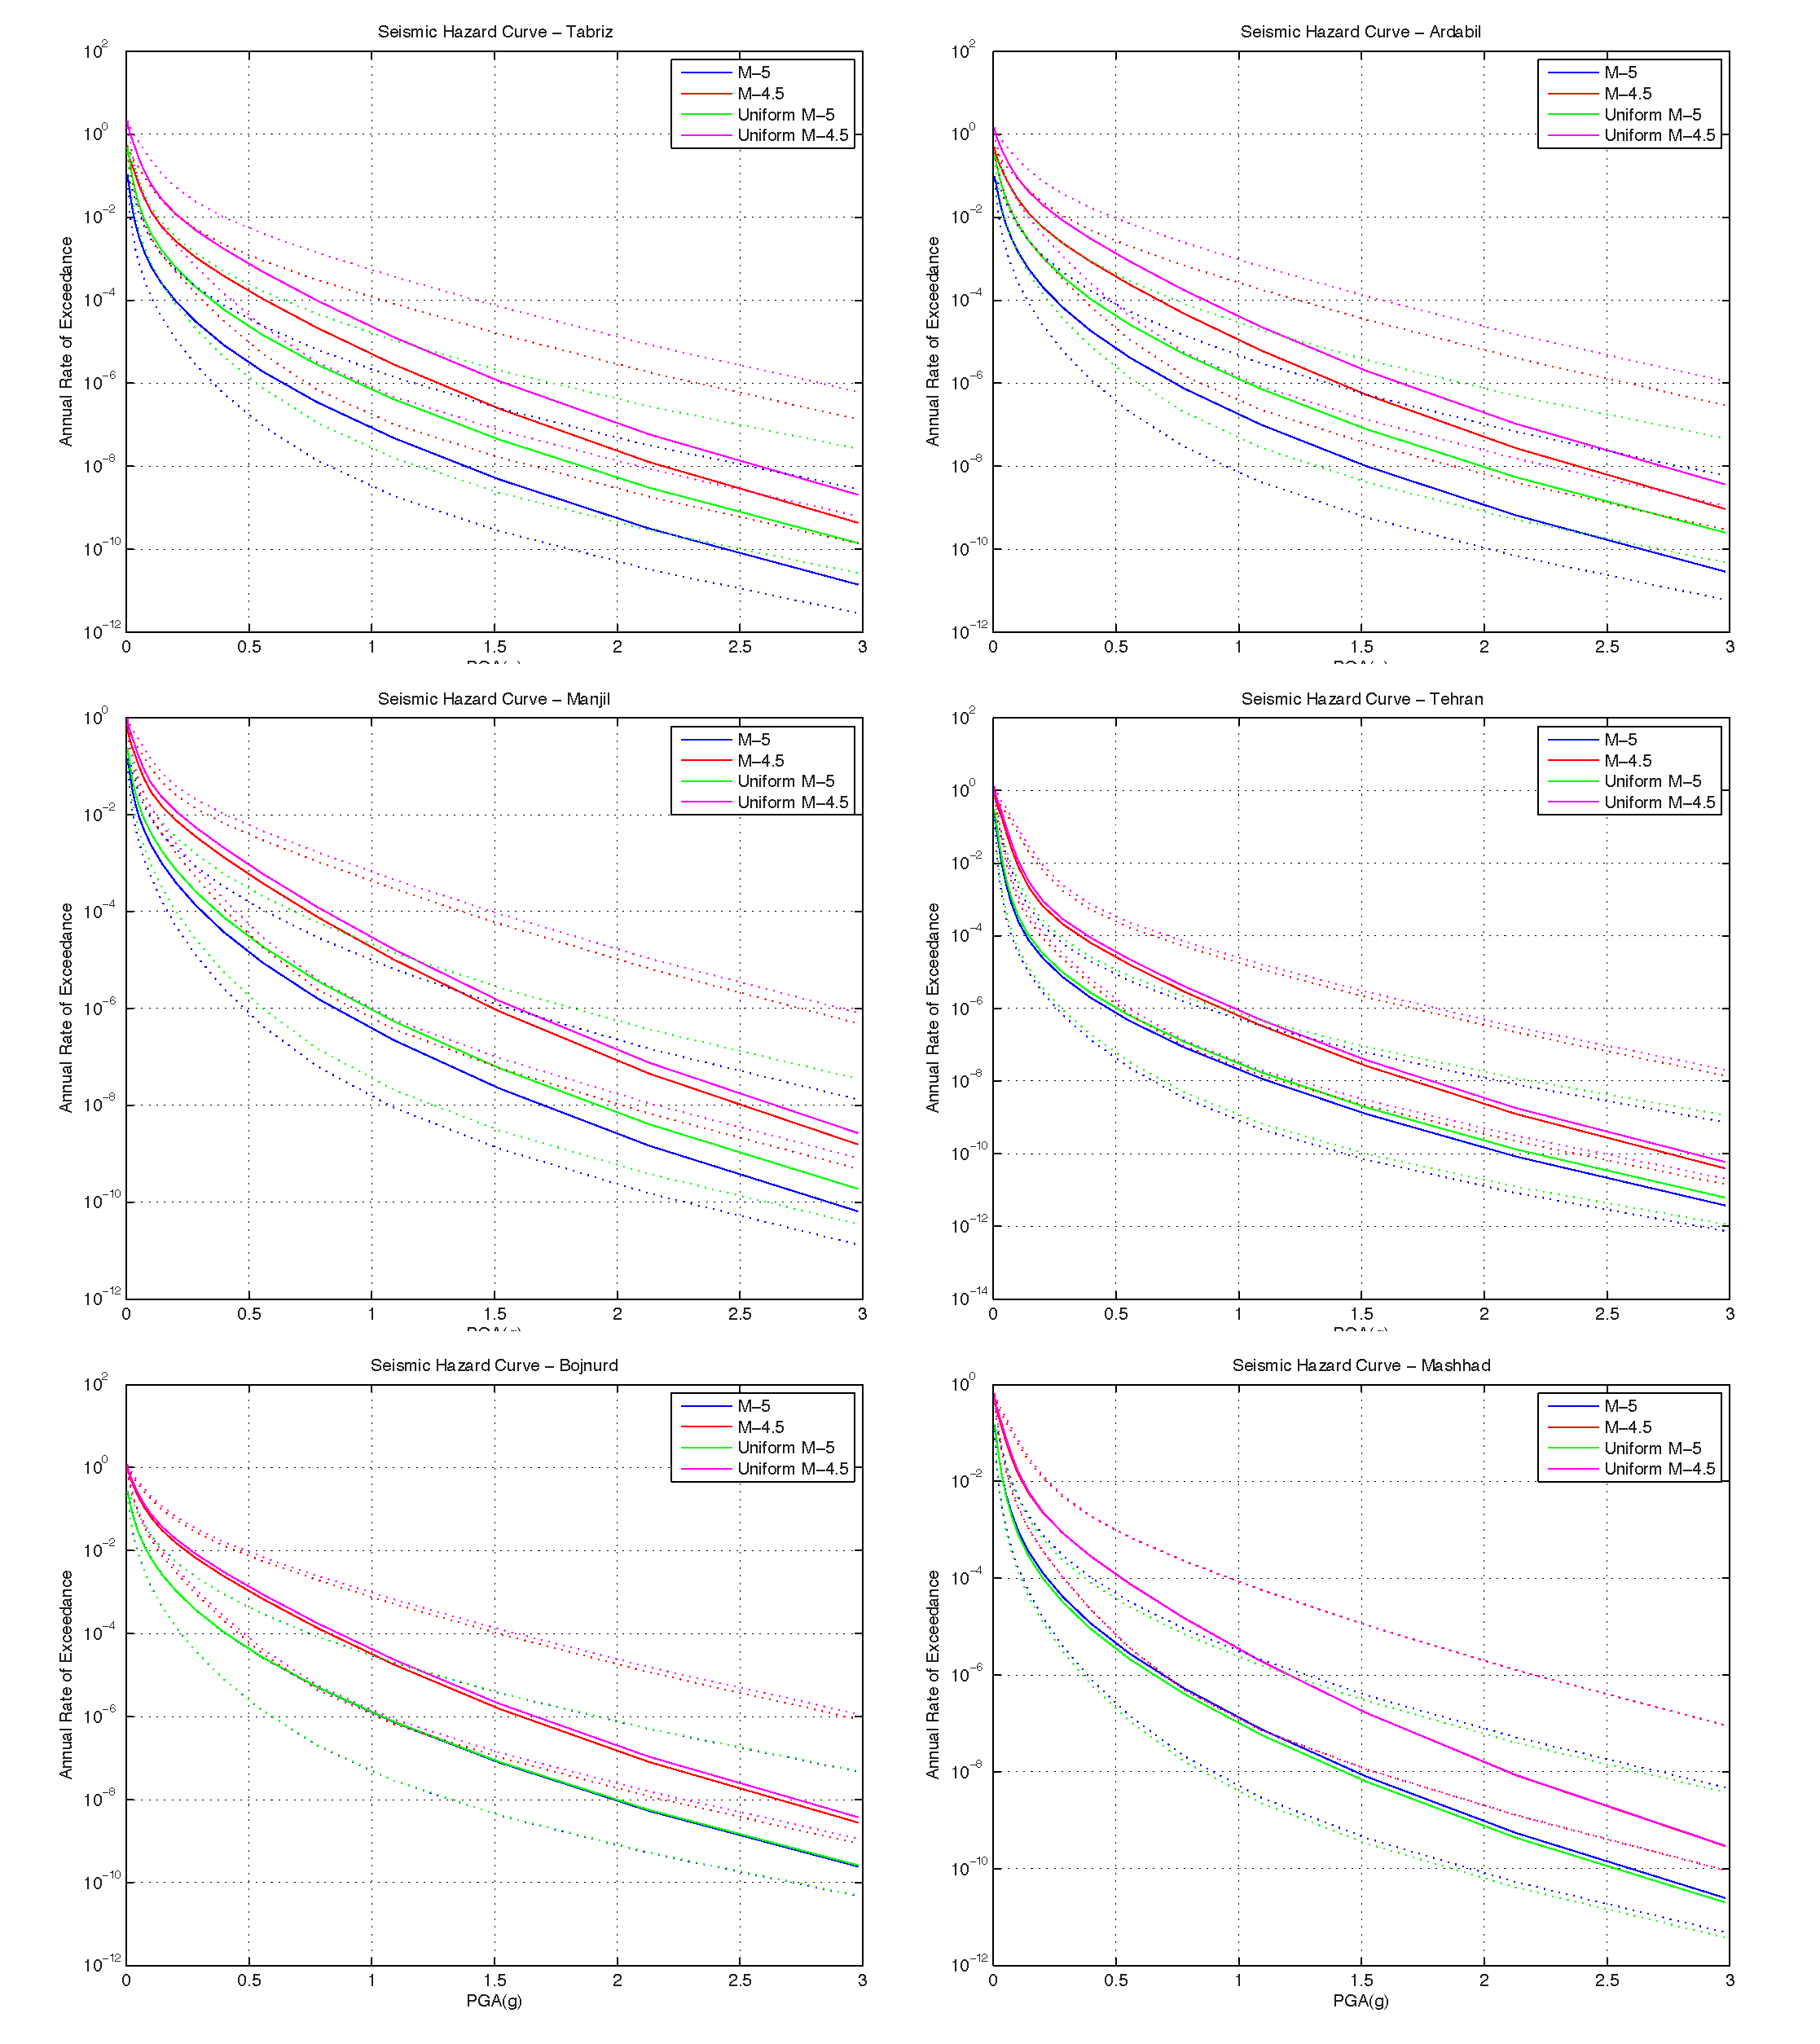
\includegraphics[scale=0.4]{figures/pdf/HazardCurve.pdf} 
\caption{Seismic Hazard Curve of Northern Cities in Iran}
\label{fig:hazardcurve}
\end{figure*}

% \subsection{Peak Ground Acceleration}

We pick the peak ground acceleration for 10\% and 2\% probability of exceedance in 50 years which correspond with 0.002 and 0.0004 annual rate of exceedance. Fig.~\ref{fig:pga_10_mean} and Fig.~\ref{fig:pga_2_mean} show the results for 10\% and 2\% probability of exceedance in 50 years, respectively. These results are according to the mean value of the attenuation relationship.

Fig.~\ref{fig:pga_10_mean_uniform} and Fig.~\ref{fig:pga_2_mean_uniform} show the results for 10\% and 2\% probability of exceedance in 50 years for the uniform model, respectively.

% -------

As discussed before the border of the study region 

Even though in this study we are interested in investigating seismic hazard study in the northern Iran, in the smoothed seismicity method we defined the border of the study region broadly enough to ensure that the seismicity outside of the border doesn't affect the study area.  In addition, the border of the influenced area should surround the area of interest as uniformly as possible \citep{Lapajne1997}. Therefore, our study region includes parts of central and eastern Iran and the Zagros tectonic seismic regions.

We calculated the $a-values$ for each cell and spatially smoothed over a grid of $0.1 \times 0.1$ in latitude and longitude. We assume magnitude increment as $\Delta_M = 0.1$. In this model, events are not assigned to specific faults and are assumed to be potential seismogenic sources, and are spatially gridded to cells.

Different correlation distances have been used in different studies, which are generally dependent on the accuracy of the location of the recorded earthquakes. \citet{Frankel1995} and \citet{Boyd2008} assumed the correlation distance to be 50 $km$. \citet{Barani2007} used distance of 25 $km$ based on previous studies that suggested the correlation function of the Alps and Apennines in Italy. \citet{Foteva2006} used 10 and 15 km in a different model. Correlation distance is a very sensitive parameter in smoothed seismic hazard maps, and it is a factor of uncertainty in earthquake location. In the Iranian earthquake catalog, the magnitude uncertainties were assumed to be in the interval of $\pm$ 0.25 magnitude units and epicentral errors of $\pm$ 30 km \citep{Zare2012}. Even though these error margins are different for different events in terms of instrumental or historical events, in this study we assumed the correlation distance as 30 km because of the lack of knowledge about other historical events. Regarding the study domain and the 0.1 grid size, the total number of source is grid sites is 11651. Even though \citet{Kalkan2004} derived the attenuation relationship up to 250 km, since \citet{Zafarani2014} used data up to 200 km to evaluate the GMPEs, we set the model to compute the ground motions at distances of less than 200 km.

Fig.~\ref{fig:10percent} and Fig.~\ref{fig:2percent} show the seismic hazard map based on background seismicity for 10\% and 2\% probability of exceedance in 50 years, respectively. The areas of large probabilistic ground motions clearly coincide with zones with a large number of events with magnitude 3 and larger.
